\documentclass[12pt]{book}

\usepackage[dvips,letterpaper,margin=0.75in,bottom=0.5in]{geometry}
\usepackage{cite}
\usepackage{slashed}
\usepackage{graphicx}
\usepackage{amsmath}
\usepackage{braket}
\begin{document}

\newcommand{\ihbar}{\ensuremath{i \hbar}}
\newcommand{\Pss}{\ensuremath{\Psi^*}}
\newcommand{\dPsidt}{\ensuremath{ \frac{\partial \Psi}{\partial t} }}
\newcommand{\dPsidx}{\ensuremath{ \frac{\partial \Psi}{\partial x} }}
\newcommand{\ddPsidx}{\ensuremath{ \frac{\partial^2 \Psi}{\partial x^2} }}
\newcommand{\dPssdt}{\ensuremath{ \frac{\partial \Psi^*}{\partial t} }}
\newcommand{\dPssdx}{\ensuremath{ \frac{\partial \Psi^*}{\partial x} }}
\newcommand{\ddPssdx}{\ensuremath{ \frac{\partial^2 \Psi^*}{\partial x^2} }}

\newcommand{\dphidt}{\ensuremath{ \frac{d \phi}{dt} }}
\newcommand{\dpsidx}{\ensuremath{ \frac{d \psi}{dx} }}
\newcommand{\ddpsidx}{\ensuremath{ \frac{d^2 \psi}{dx^2} }}


\title{PHY 115A \\ Lecture Notes: \\ 
Time-Independent Schr\"odinger Equation \\
(Griffith's Chapter 2)}
\author{Michael Mulhearn}

\maketitle

\setcounter{chapter}{1}
\chapter{Time-Independent Schr\"odinger Equation}

\section{Stationary States}

Here's our summary of Griffiths section 2.1:

We attempt to solve the Schr\"odinger Equation:
\begin{equation}
\label{eqn:se}
\ihbar \, \dPsidt \; = \; - \frac{\hbar^2}{2 m} \; \ddPsidx \, + \, V \, \Psi
\end{equation}
in the case that the potential V(x) is not a function of $t$.  We will try to find a solution under the assumption that $\Psi(x,t)$ is separable:
\begin{equation}
\Psi(x,t) \; = \; \psi(x) \,\phi(t)
\end{equation}
which yields:
\begin{eqnarray*}
\ihbar \, \psi \dphidt \; &=& \; - \frac{\hbar^2}{2 m} \; \phi \ddpsidx \, + \, V \, \Psi\\
\ihbar \, \frac{1}{\phi(t)} \dphidt \; &=& \; - \frac{\hbar^2}{2 m} \; \frac{1}{\psi(x)}\ddpsidx \, + \, V(x)\\
\end{eqnarray*}
As the LHS is a function of $t$ only, and the RHS a function of $x$ only, both sides must be constant wrt $t$ and $x$ respectively.  We'll call that constant $E$, and solve for $\phi(t)$:
\begin{eqnarray*}
\ihbar \, \frac{1}{\phi(t)} \dphidt \; &=& E\\
\int \frac{d\phi}{\phi(t)}  \; &=& -\frac{iE}{\hbar} \int dt\\
\ln \phi &=& -\frac{iEt}{\hbar}\\
\phi(t) &=& \exp(-\frac{iEt}{\hbar})\\
\end{eqnarray*}
The remaining equation is for $\psi(x)$ only
\begin{eqnarray*}
- \frac{\hbar^2}{2 m} \; \ddpsidx \, + \, V \, \psi &=& E \psi\\
\end{eqnarray*}
and is called the Time-Independent Schr\"odinger Equation (TISE), often just called the Schr\"odinger Equation when the meaning is clear.

In classical mechanics, the total energy (kinetic plus potential) is called the Hamiltonian:
\begin{equation*}
H(x,p) = \frac{p^2}{2m} + V(x)
\end{equation*}
We can construct the corresponding operator in quantum mechanics by substituting 
\begin{eqnarray*}
x &\to& \hat{x} = x \\
p &\to& \hat{p} = -i\hbar \frac{\partial}{\partial x} \\
\end{eqnarray*}
to calculate:
\begin{equation}
\hat{H} = H(\hat{x}, \hat{p})= -\frac{\hbar^2}{2m}\,\frac{\partial^2}{\partial x^2} + V(x)
\end{equation}
with which we can write the TISE as:
\begin{equation}
\label{eqn:htise}
\hat{H} \, \psi(x) = E \, \psi(x)
\end{equation}
We'll demonstrate later the following boundary conditions on $\psi(x)$:
\begin{itemize}
\item $\psi(x)$ is always continuous.
\item $d\psi/dx$ is continuous except where the potential is infinite.
\end{itemize}
Note that these conditions do not apply to $\Psi(x,t)$ no $\partial \Psi / \partial x$ which need not be continuous.

\noindent
Some observations left as exercises (See Griffith's problems 2.1 and 2.2)
\begin{itemize}
\item For normalizable solutions, we must the separation constant E real.
\item $\psi(x)$ can always be taken real.
\item If $V(x)$ is an even function, than $\psi(x)$ can be taken as even or odd.
\item $E$ must be greater than the minimum value of $V(x)$.
\end{itemize}






\noindent
The separable solutions are important solutions because:
\begin{itemize}
\item They represent {\bf stationary states}:  even though the ``full'' wave function
\begin{equation*}
\Psi(x,t) = \phi(t) \, \psi(x) = e^{-iEt/h} \, \psi(x)
\end{equation*}
has a time dependence, the probability density is constant with time:
\begin{eqnarray*}
|\Psi(x,t)|^2 &=& \left(e^{-iEt/h} \, \psi(x)\right)^* \; \left(e^{-iEt/h} \, \psi(x)\right)\\[8pt]
&=& e^{iEt/h-iEt/h} \, \psi^*(x) \psi(x)\\[8pt]
&=& | \psi(x) |^2
\end{eqnarray*}
This means that every expectation value is constant wrt time as well.  It also follows that:
\begin{equation*}
\int_{-\infty}^{+\infty}\, |\psi(x)|^2 dx = 1\\
\end{equation*}


\item They represent {\bf states of definite total energy:} the expectation value for the total energy of a separable solution is:
\begin{eqnarray*}
\braket{E} &=& \int_{-\infty}^{+\infty}\, \Psi^*(x,t) \, \hat{H} \, \Psi(x,t) \; dx \\[8pt]
           &=& \int_{-\infty}^{+\infty}\, \psi^*(x) \, \hat{H} \, \psi(x) \; dx \\[8pt]
           &=& \int_{-\infty}^{+\infty}\, \psi^*(x) \, E \, \psi(x) \; dx \\[8pt]
           &=& E \int_{-\infty}^{+\infty}\, |\psi(x)| \; dx \\[8pt]
           &=& E           
\end{eqnarray*}
Remember that we just chose $E$ as the symbol for the constant value when using separation of variables.  This shows why we choose $E$, as that constant is the expectation value of the total energy.  Now calculate in a similar fashion:
\begin{eqnarray*}
\braket{E^2} &=& \int_{-\infty}^{+\infty}\, \Psi^*(x) \, \hat{H}^2 \, \Psi(x) \; dx \\[8pt]
           &=& E^2
\end{eqnarray*}
From which it follows:
\begin{equation*}
\sigma^2_H = \braket<E^2> - \braket{E}^2 = E^2 - E^2 = 0
\end{equation*}
This means that every measurement of the particles total energy will yield the result $E$.
\item There is more, but (unlike Griffiths) we will leave those features for later.
\end{itemize}

\section{Infinite Square Well}

Next we will turn our attention to the infinite square well:
\begin{equation}
V(x) = 
\begin{cases}    
   0 & 0 \leq x \leq a \\
   +\infty & {\rm otherwise} \\
\end{cases}   
\end{equation}
By setting $V(x) = +\infty$ outside the well, we just mean $\Psi(x,t)=0$ in that region, and not anything more.  We also see that for normalizable solutions, we must have $E>0$.

We are looking for the stationary states that solve the TISE:
\begin{eqnarray*}
\hat{H} \, \psi(x) \; &=& \; E \, \psi(x) \\
\end{eqnarray*}
Inside the well we have:
\begin{eqnarray*}
-\frac{\hbar^2}{2m}\,\frac{\partial^2\psi}{\partial x^2} &=& \; E \, \psi(x) \\[8pt]
\ddpsidx &=& -k^2 \psi \\
\end{eqnarray*}
where
\begin{eqnarray*}
k &\equiv& \frac{\sqrt{2mE}}{\hbar} \\
\end{eqnarray*}
Taking $\psi(x)$ to be real, the solutions are:
\begin{equation*}
\psi(x) = A \sin(kx) + B \cos(ks)
\end{equation*}
And the continuity requirements on $\psi(x)$ imply:
\begin{equation*}
\psi(0) = \psi(a) = 0.
\end{equation*}
Why is there no continuity condition on $d\psi/dx$?  Applying the conditions:
\begin{equation*}
\psi(0) = A \sin(0) + B \cos(0) = B = 0
\end{equation*}
So now:
\begin{equation*}
\psi(x) = A \sin(kx) 
\end{equation*}
And applying the other condition:
\begin{eqnarray*}
\psi(a)  &=& A \sin(ka) = 0 \\
\sin(ka) &=& 0 \\
\end{eqnarray*}
Where in the last step we have used $A \neq 0$ because $A=0$ implies $\psi(x)=0$ a non-normalizable solution.  The sin function is zero for any integer value of pi, so:
\begin{eqnarray*}
ka &=& n \pi \\[12pt]
k_n&=&\frac{n\pi}{a}
\end{eqnarray*}
where $n$ is any integer.  The normalization condition implies:

\begin{eqnarray*}
\int_{-\infty}^{+\infty} \; |\psi(x)|^2 \, dx &=& 1 \\
1 &=& \int_{0}^{a} \; |A \, \sin(k_n x)|^2 \, dx \\
1 &=& |A|^2 \int_{0}^{a} \; \sin(k_n x)|^2 \, dx \\
1 &=& |A|^2 \; \frac{a}{2} \\
|A|^2 &=& \frac{2}{a} \\
\end{eqnarray*}
As the phase of $A$ doesn't matter for the purposes of normalization, we choose it to be positive real
\begin{eqnarray*}
\int_{-\infty}^{+\infty} \; |\psi(x)|^2 \, dx &=& 1 \\
A &=& \sqrt{\frac{2}{a}} \\
\end{eqnarray*}
So at last we have an infinite number of solutions to the TISE:

\begin{equation}
\psi_n(x) = \sqrt{\frac{2}{a}}\sin(k_n x)
\end{equation}
where
\begin{eqnarray*}
k_n&=&\frac{n\pi}{a}
\end{eqnarray*}
In principle, $n$ can be any integer, but for $n=0$ we get the unnormalizable wave function $\psi(x)=0$ and so we omit $n=0$.  We note also that:
\begin{eqnarray*}
\psi_{-n}(x) = \sqrt{\frac{2}{a}} \sin(k_{-n}x) = \sqrt{\frac{2}{a}} \sin(-k_{n}x) = -\sqrt{\frac{2}{a}} \sin(k_{n}x) = -\psi_{n}(x)
\end{eqnarray*}


So $\psi_{-n}$ differs from $\psi_{n}$ only by a phase factor $-1$ and therefore adds nothing (recall that we simply chose $A$ to be positive and real).  So we can omit negative values of $n$ as well.  That leaves us with:
\begin{equation*}
n = 1,2,3,\ldots
\end{equation*}

Recalling our definition for $k$, the definite total energy $E_n$ of stationary state $\psi_n$ is given by:
\begin{eqnarray*}
k_n &=& \frac{n\pi}{a} = \frac{\sqrt{2mE_n}}{\hbar}\\[10pt]
E_n &=& \frac{\hbar^2k_n^2}{2m}= \frac{n^2 \pi^2 \hbar^2}{2ma^2}\\
\end{eqnarray*}

You may recognize the $\psi_n(x)$ as ... 

\section{The Fourier Series as a Vector Space}

In this section, we'll see how the Fourier Series defines a Vector Space.

We'll start by definining the properties of a vector space in the familiar setting of the 3-D Euclidean Vectors.

\subsection{Euclidean Vector Space}

We are going to be introducing the concept of a vector space, so let's review this in the context of ordinary euclidean vectors in three dimensional space.  Such a vector is completely specified by its displacement in each spatial direction.  Let's look at this familiar picture a bit formally, to prepare us to apply it in a less intuitive (but mathematically equivalent) setting.  

We have {\bf vector addition} with the following properties:
\begin{itemize}
\item {\bf Closure under addition:} The addition of two vectors is another vector:
$$\vec{u} + \vec{v} = \vec{w}$$
\item {\bf Commutative}:  
$$\vec{u} + \vec{v} = \vec{v} + \vec{u}$$
\item {\bf Associated}:  
$$\vec{u} + (\vec{v} + \vec{w}) = (\vec{u} + \vec{v}) + \vec{w} $$
\item {\bf Zero}:  There is the vector 0 with:
$$\vec{u} + 0 = \vec{u} $$
\item {\bf Inverse vector}:  For every $\vec{u}$ there is $(-\vec{u})$ s.t.:
$$\vec{u} + (-\vec{u}) = 0 $$
\end{itemize}

We have {\bf scalar multiplication} with the following properties:
\begin{itemize}
\item {\bf Closure under scalar multiplication:} The product of a scalar and a vector is another vector:
$$a \vec{u} = \vec{w}$$
\item {\bf Distributive}:  
$$a(\vec{u} + \vec{v}) = a\vec{u} + a\vec{v}$$
\item {\bf Associative}:  
$$a(b\vec{u}) = (ab)\vec{u})$$
\item {\bf Multiplication by one}:
$$1\vec{u}) = \vec{u}$$
\item {\bf Multiplication by zero}:
$$0\vec{u}) = 0$$
\end{itemize}

We also have the dot product, but this is called an {\bf inner product} within an $n-dimensional$ vector space:
\begin{displaymath}
\vec{v} \cdot \vec{w} = v_x w_x + v_y w_y + v_z w_z 
\end{displaymath}
You already know how to do this for ordinary vectors.  In other settings, we use the more general term {\em inner product}.  To describe any vector we need a set of {\em basis vectors}, in this case $\hat{x}$, $\hat{y}$, and $\hat{z}$.  These basis vectors are orthogonal:
\begin{displaymath}
\hat{x} \cdot \hat{y} = \hat{y} \cdot \hat{z} = \hat{z} \cdot \hat{x} = 0
\end{displaymath}
and normalized:
\begin{displaymath}
\hat{x} \cdot \hat{x} = \hat{y} \cdot \hat{y} = \hat{z} \cdot \hat{z} = 1.
\end{displaymath}
When the basis vectors have both of these properties, we call them {\em orthonormal}.

For any possible vector $\vec{v}$, we can calculate its component in the direction of each basis vector by calculating the inner product:
\begin{eqnarray*}
v_x = \vec{v} \cdot \hat{x} \\
v_y = \vec{v} \cdot \hat{y} \\
v_z = \vec{v} \cdot \hat{z} \\
\end{eqnarray*}
We say that the basis vectors $\hat{x}$, $\hat{y}$, and $\hat{z}$ are "complete", because specifying the values of $v_x$, $v_y$, and $v_z$ completely describes the vector $v$.  The set of basis vectors $\hat{x}$ and $\hat{z}$ are orthonormal, but they are not complete in three dimensional space, because there are vectors which we cannot write using only these two directions.  For instance, there are no possible values for $v_x$ and $v_z$
which make
\begin{eqnarray*}
 \vec{v_1} = v_x \hat{x} + v_z \hat{z}
\end{eqnarray*}
equal to the vector
\begin{eqnarray*}
 \vec{v_2} = 3 \hat{x} + 2 \hat{y} + 7 \hat{z}.
\end{eqnarray*}
Orthogonality and completeness are intimately related.  In Euclidean vector space, any three orthogonal vectors must be complete.
 
\section{The Fourier Series}

Using the language of vector spaces, the Fourier Theorem states that the sines and cosines form a complete orthonormal basis for any periodic function.  

The vectors in this vector space are periodic functions.  Vector addition of the vectors $f(x)$ and $g(x)$ is just $f(x) + g(x)$ which is another vector.  Scalar multiplication is just multiplying a function $f(x)$ by a scalar $a$ to get a new function $a f(x)$.  The other properties of vector addition and scalar multiplication easily follow from the corresponding rules of ordinary addition and multiplication.

We need to define the inner product. If we restrict ourselves to {\bf real} functions of $x$ with period $a$, the inner product between any two functions $f(x)$ and $g(x)$ is defined to be the integral:
\begin{equation}
\braket{f,g} \equiv \int_{-\frac{a}{2}}^{\frac{a}{2}} f(x) \, g(x) \, dx
\end{equation}
The basis vectors are the sine and cosine functions
\begin{eqnarray}
s_n(x) \equiv \sqrt{\frac{2}{a}}\,\sin\left(\frac{2\pi n}{a} \, x \right)\\
c_n(x) \equiv \sqrt{\frac{2}{a}}\,\cos\left(\frac{2\pi n}{a} \, x \right)
\end{eqnarray}
which are defined for
\begin{eqnarray}
n = 0,1,2,3,...
\end{eqnarray}
except that $s_0(0)=0$ is not normalizable.  We'll leave it as an exercise to show that:
\begin{eqnarray}
\braket{s_n,s_m} &=& \frac{2}{a} \int_{-\frac{a}{2}}^{\frac{a}{2}} 
\sin\left(\frac{2\pi n}{a} \, x \right) \sin\left(\frac{2\pi m}{a} \, x \right) \, dx = \delta_{nm} \;\;\;\;\; (n \neq 0) \notag\\[8pt]
\braket{c_n, c_m} &=& \frac{2}{a} \int_{-\frac{a}{2}}^{\frac{a}{2}} 
\cos\left(\frac{2\pi n}{a} \, x \right) \cos\left(\frac{2\pi m}{a} \, x \right) \, dx = \delta_{nm}\notag\\[8pt]
\braket{s_n, c_m} &=& \frac{2}{a} \int_{-\frac{a}{2}}^{\frac{a}{2}} 
\sin\left(\frac{2\pi n}{a} \, x \right) \cos\left(\frac{2\pi m}{a} \, x \right) \, dx = 0 \notag\\
\end{eqnarray}
where for compact notation we will use the Kronecker delta symbol:
\begin{displaymath}
\delta_{nm} =  
\left\{
	\begin{array}{ll}
		1  & \mbox{if } n=m \\
		0 & \mbox{otherwise}
	\end{array}
\right.
\end{displaymath}

Fourier's Theorem states that these orthonormal basis functions are complete for the vector space of periodic functions with period $a$.  That is, if $f(x)$ has the property that:
$$f(x) = f(x+a)$$
then $f(x)$ can be written as a sum of the orthonormal basis vectors:
\begin{equation}
f(x) \; = \; \sum_{n=0}^{\infty}  A_n \, c_n(x)  \; \; + \; \; \sum_{n=1}^{\infty} B_n \, s_n(x) \label{eqn:bfs}
\end{equation}
or explicitly in terms of sine and cosine functions:
\begin{equation}
f(x) = \sqrt{\frac{2}{a}} \, \sum_{n=0}^{\infty}  A_n \, \cos\left(\frac{2\pi n}{L} \, x \right) + \sqrt{\frac{2}{a}} \, \sum_{n=1}^{\infty} B_n \, \sin\left(\frac{2\pi n}{L} \, x \right)  s_n(x) \label{eqn:lfs}
\end{equation}

The values $A_n$ and $B_n$ are called {\em Fourier coefficients}.  Technically the $N$th term in the Fourier Series refers to the approximation for $f(x)$ from the first $N$ terms in the infinite sum above, and we say that the Fourier Series converges to the function $f(x)$.  The demonstration of completeness is optional reading, available in the Appendix.

\begin{figure}[thb]
\begin{center}
{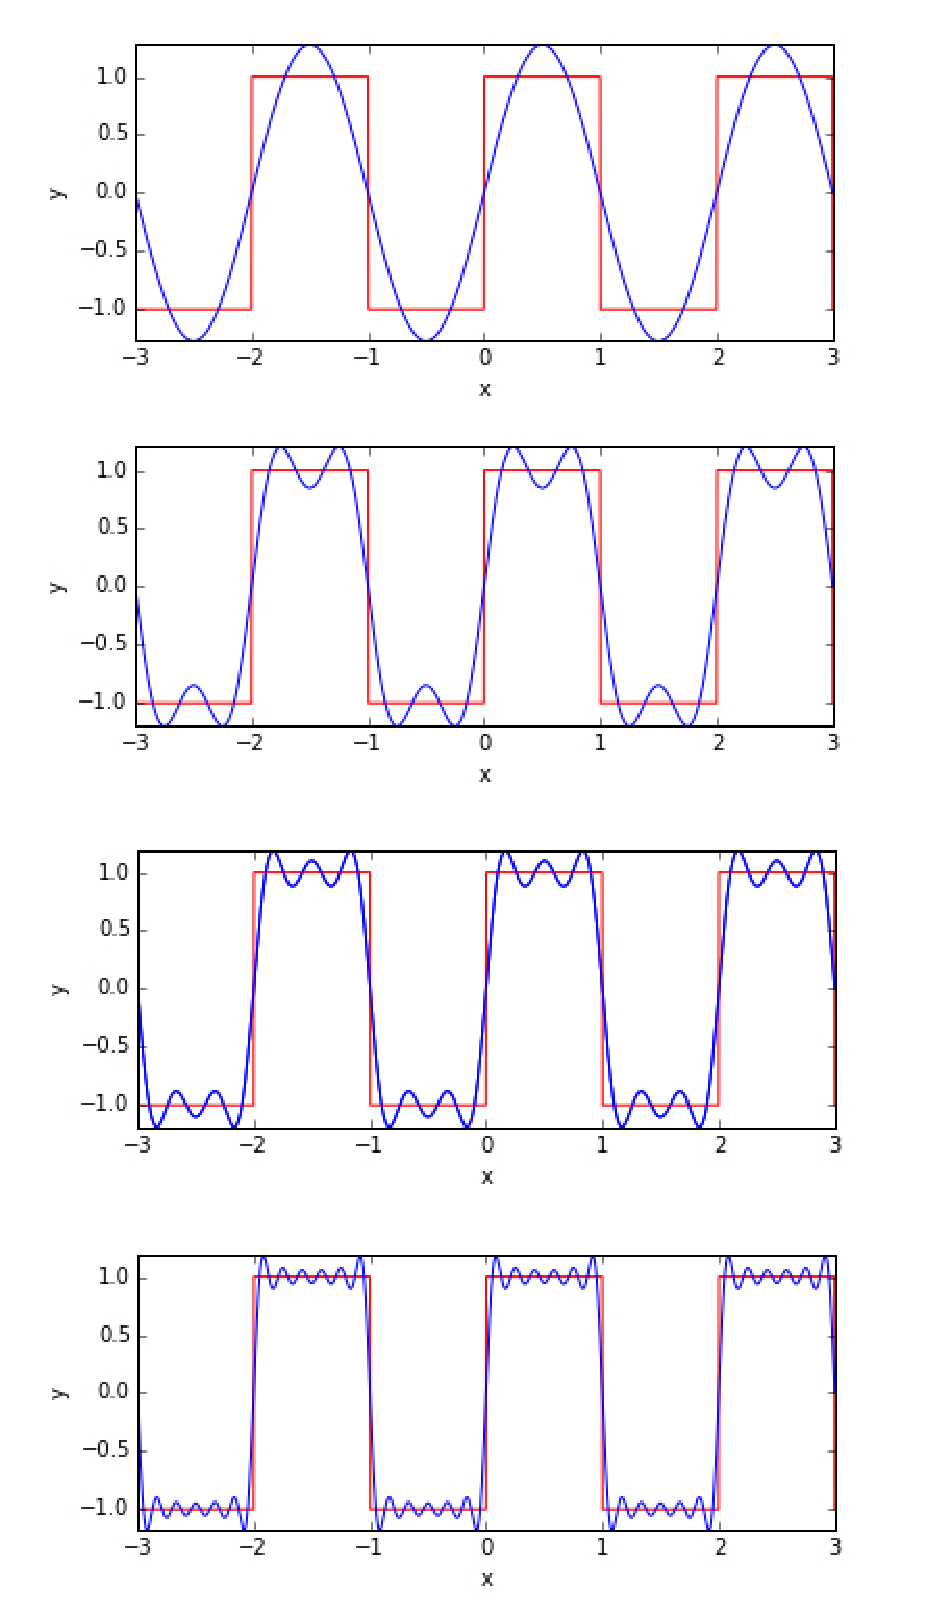
\includegraphics[width=0.40\textwidth]{figs/fsall.pdf}}
\end{center}
\caption{\label{fig:fall} The Fourier Series for a step function including one term, three terms, five terms, and nineteen terms.  The Fourier Theorem states that the series will converge, reproducing the original function, as the number of terms approaches infinity.}
\end{figure}

For a visual example of the Fourier Series, the first terms of the Fourier Series for a step function are shown in Fig.~\ref{fig:fall}.  

\section{Determining the Fourier Coefficients}
\label{sect:coeff}

Just as in the vector analogy, we can determine the Fourier coefficients of a function $f$ by computing the inner products:
\begin{eqnarray*}
A_n = \braket{c_n, f} \\
B_n = \braket{s_n, f}
\end{eqnarray*}
or, in terms of the inner product integrals and sine and cosine functions:
\begin{eqnarray}
A_n &=& \sqrt{\frac{2}{a}} \int_{-\frac{a}{2}}^{\frac{a}{2}} 
f(x) \cos\left(\frac{2\pi n}{a} \, x \right) \, dx \label{eqn:fca} \\
B_n &=& \sqrt{\frac{2}{a}} \int_{-\frac{a}{2}}^{\frac{a}{2}} 
f(x) \sin\left(\frac{2\pi n}{a} \, x \right) \, dx
\end{eqnarray}

The inner product determines the correct coefficients only because the basis functions are complete and orthonormal.  To see how this works, start with the completeness equation but replace $n$ with $m$ for clarity later:
\begin{equation*}
f(x) \; = \; \sum_{m=0}^{\infty}  A_m \, c_m(x)  \; \; + \; \; \sum_{m=1}^{\infty} B_m \, s_m(x) 
\end{equation*}
Then calculate:
\begin{eqnarray*}
\braket{c_n, f} \; &=& \; \sum_{m=0}^{\infty}  A_m \, \braket{c_n, c_m}  \; \; + \; \; \sum_{m=1}^{\infty} B_m \, \braket{c_m, s_m} \\[8pt]
 &=& \; \sum_{m=0}^{\infty}  A_m \; \delta_{nm}  \; \; + \; \; \sum_{m=1}^{\infty} B_m \; 0 \\[8pt]
\braket{c_n, f} \; &=& A_n \\
\end{eqnarray*}
Note that the last step follows from the fact that, because of the $\delta_{nm}$ in the product, the only non-zero value in the sum across $m$ is the term for $m=n$.  It is left as an exercise to work this out for $\braket{s_n, f}$.

\section{The Half-Period Fourier Series}

Suppose a function f(x) is even, i.e.:
$$f(-x) = f(x)$$
a function g(x) is odd, i.e.:
$$g(-x) = -g(x)$$.
Then the following integral vanishes:
\begin{alignat*}{2}
\int_{-a}^{a} 
f(x) g(x) dx &=  &\int_{-a}^{0} f(x) g(x) dx + \int_{0}^{a} f(x) g(x) dx\\[14pt]
 &=&\int_{0}^{a} f(-x) g(-x) dx + \int_{0}^{a} f(x) g(x) dx\\
 &=&\int_{0}^{a} f(-x) g(-x) dx + \int_{0}^{a} f(x) g(x) dx\\
 &=& 0 \\
\end{alignat*}

  



Suppose f(x) is even, then:
\begin{eqnarray*}
A_n &=& \braket{s_n,f} \\
    &=& \sqrt{\frac{2}{a}} \int_{-\frac{a}{2}}^{\frac{a}{2}} 
f(x) \cos\left(\frac{2\pi n}{a} \, x \right) \, dx \label{eqn:fca} \\
\sqrt{\frac{2}{a}} \int_{0}^{\frac{a}{2}} 
f(x) \cos\left(\frac{2\pi n}{a} \, x \right) \, dx \label{eqn:fca} \\
\end{eqnarray*}

A function $f(x)$ is odd, i.e.:
$$f(-x) = -f(x)$$
with 


\appendix

\chapter{Proofs of Completeness of Trigonometric Functions}


\subsection{The Dirac Delta Function}

These proofs make extensive use of the Dirac delta function, $\delta(x)$, which is zero everywhere but at $x=0$, where it is infinite.  Mathematically, the delta function only makes formal sense inside an integral, where it has the following defining properties:
\begin{eqnarray}
\int_{-\infty}^{\infty} f(x') \, \delta(x-x') \, dx' &=& f(x) \\
\int_{-\infty}^{\infty} \delta(x) \, dx &=& 1 \label{eqn:norm}
 \end{eqnarray}
The delta function simply picks out from the integral the one value of the integrand which makes the argument of the delta function zero.  This makes intuitive sense, because the delta function is zero everywhere else.  The second equation shows the normalization of the delta function, which follows from the first if you take $f(x)=1$.





\subsection{The completeness of the sines and cosines}

\begin{figure}[thb]
\begin{center}
{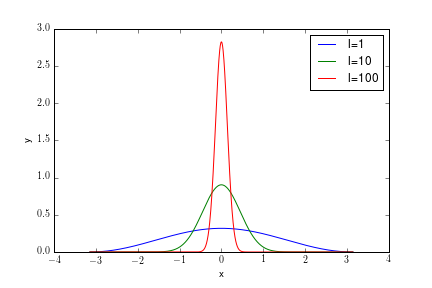
\includegraphics[width=0.40\textwidth]{figs/hk.png}}
\end{center}
\caption{\label{fig:hl} The function $h_\ell(x)$ for increasingly large values of $\ell$.}
\end{figure}

\noindent
To demonstrate the completeness of sines and cosines\footnote{This proof taken from http://web.mit.edu/jorloff/www/18.03-esg/notes/fourier-complete.pdf} we construct a peculiar but useful set of functions defined for $\ell=1,2,3,...$:
\begin{displaymath}
h_\ell(x) = c_\ell \left(\frac{1 + \cos(x)}{2}\right)^\ell
\end{displaymath}
We chose each factor $c_\ell$ such that:
\begin{displaymath}
\int_{-\pi}^{\pi} h_\ell(x) = 1
\end{displaymath}
The shape of $h_\ell$ is shown in Fig.~\ref{fig:hl}.  As $\ell$ increases, $h_\ell$ becomes more and more narrow at $x=0$, while the normalization is as in Equation~\ref{eqn:norm}.  It looks more and more like the delta function:
\begin{displaymath}
\lim_{\ell \to \infty} h_\ell(x) = \delta(x)
\end{displaymath}
It has one other important feature:  $h_\ell(x)$ is simply a sum of cosines of $nx$ with coefficients that don't depend on $x$.  To see how this can be, note that we can always turn a product of cosines into a sum via the trigonometric identity:
\begin{displaymath}
\cos \alpha \cos \beta = \frac{1}{2} \{\cos(\alpha - \beta) + \cos(\alpha + \beta)\}.
\end{displaymath}
So, for instance, we can write:
\begin{eqnarray*}
h_2(x) &=& \frac{c_2}{4} + \frac{c_2\cos(x)}{2}+\frac{c_2\cos^2(x)}{4} \\
           &=& \frac{c_2}{4} + \frac{c_2\cos(x)}{2}+\frac{c_2\cos(2x)}{8}
\end{eqnarray*}
This property implies that the function $h_\ell(x-a)$ for some constant $a$ is simply a sum of {\em both} sines and cosines of $nx$ with coefficients that don't depend on $x$, as:
\begin{displaymath}
\cos(nx-na) = \cos(nx)\cos(na) + \sin(nx)\sin(na).
\end{displaymath}

With this technology in hand we are ready to demonstrate the completeness of the sines and cosines.   
For simplicity, it suffices to consider only functions with period $L=2\pi$ (i.e. $k_n=n$).  The general case can then be inferred by transformation of coordinates.  Consider a real function $f(x)$ which is periodic for $L=2\pi$.  For now just define the function $F(x)$ to be the infinite series:
\begin{eqnarray}
F(x) \equiv a_0 + \sum_{n=1}^{\infty}  \left\{ a_n \, \cos(n x ) + b_n \, \sin(n x ) \right\}.
\end{eqnarray}
This is the compact form of the Fourier Series for this special case $L=2\pi$, so $k_n = n$.
We assume the coefficients are determined in the usual way:
\begin{eqnarray*}
a_n &=& \frac{2}{L} \int_{-\frac{L}{2}}^{\frac{L}{2}} 
f(x) \cos(n x) \, dx  \\
b_n &=& \frac{2}{L} \int_{-\frac{L}{2}}^{\frac{L}{2}} 
f(x) \sin(n x) \, dx.
\end{eqnarray*}
We need to show that $F(x) = f(x)$, or 
\begin{displaymath}
g(x) = F(x) - f(x) = 0
\end{displaymath}
The proof hinges on the fact that $F(x)$ and $f(x)$ have the same Fourier coefficients, so that:
\begin{eqnarray*}
\int_{-\pi}^{\pi} g(x) \sin(nx) dx &=& \int_{-\pi}^{\pi} F(x) \sin(nx) dx -  \int_{-\pi}^{\pi} f(x) \sin(nx) dx \\
&=& b_n - b_n \\
&=& 0 \\
\int_{-\pi}^{\pi} g(x) \cos(nx) dx &=& \int_{-\pi}^{\pi} F(x) \cos(nx) dx -  \int_{-\pi}^{\pi} f(x) \cos(nx) dx \\
&=& a_n - a_n \\
&=& 0 
\end{eqnarray*}
This shows that the integral of $g(x)$ times any sine or cosine is zero.  But our special function $h_\ell(x-a)$ function is just a sum of sines and cosines of $nx$ for any value of $a$.  This means that:
\begin{eqnarray*}
\int_{-\pi}^{\pi} h_\ell(x-a) g(x) dx &=& 0 \\
\end{eqnarray*}
If we take the limit as $\ell \to \infty$, we obtain:
\begin{eqnarray*}
\int_{-\pi}^{\pi} \delta(x-a) g(x) dx &=& 0 \\
g(a) &=& 0 \\
\end{eqnarray*}
Since this is true for any value of $a$, we have $g(x) = 0$ and so $F(x) = f(x)$.

\subsection{The orthogonality and completeness of the complex exponential function}

The first thing we need to show is that:
\begin{equation} \label{eqn:delta}
\frac{1}{2\pi} \int_{-\infty}^{\infty} \exp(ikx) \, dk = \delta(x)
\end{equation}
To see this we first calculate:
\begin{eqnarray*} \label{eqn:delta}
\frac{1}{2\pi} \int_{-a}^{a} \exp(ikx) \, dk &=& \frac{1}{2\pi} \, \frac{\exp(iax)-\exp(-iax)}{ix}\\
&=& \frac{1}{\pi} \, \frac{\sin(ax)}{x} \\
&=& \frac{a}{\pi} \, {\rm sinc}(ax)
\end{eqnarray*}
An integration shows that:
\begin{eqnarray}
\int_{-\infty}^{\infty} \frac{a}{\pi} \, {\rm sinc}(ax) \, dx = 1
\end{eqnarray}
exactly as needed for Equation~\ref{eqn:norm}.

Fig.~\ref{fig:sinc} shows that this function peaks at zero and becomes more and more narrow for progressively larger values of $a$.  Since it has the correct normalization, we conclude that:
\begin{eqnarray*}
\frac{1}{2\pi} \int_{-\infty}^{\infty} \exp(ikx) \, dk &=& \lim_{a\to\infty} \frac{1}{2\pi} \int_{-a}^{a} \exp(ikx) \, dk \\
&=& \lim_{a\to\infty} \frac{a}{\pi} \, {\rm sinc}(ax) \\ 
&=& \delta(x)
\end{eqnarray*}

\begin{figure}[thb]
\begin{center}
{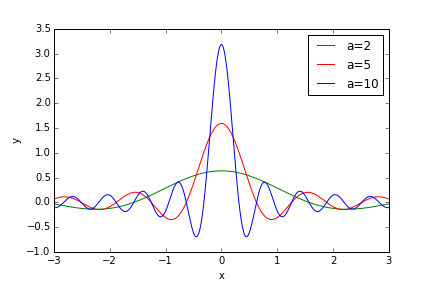
\includegraphics[width=0.40\textwidth]{figs/sinc.png}}
\end{center}
\caption{\label{fig:sinc} The function $a \, {\rm sinc}(ax)/\pi$ for progressively larger values of $a$.  As $a \to \infty$, this function approaches the delta function $\delta(x)$.}
\end{figure}

We are now fully equip to show that the complex exponential functions:
\begin{equation*}
e_k = \frac{1}{\sqrt{2\pi}} \exp(i k x)
\end{equation*}
are orthonormal.  Calculating the inner product
\begin{eqnarray*}
\braket{e_k, e_{k'}} &=& \int_{-\infty}^{\infty} \frac{1}{\sqrt{2 \pi}}  \exp(-ikx) \frac{1}{\sqrt{2 \pi}}  \exp(ik'x) \, dx \\
                               &=& \frac{1}{2 \pi} \int_{-\infty}^{\infty} \exp\{i(k'-k)x\} \, dx \\
                               &=& \delta(k-k')
\end{eqnarray*}
where we have used Equation~\ref{eqn:delta} but with the roles of $x$ and $k$ exchanged.
To prove completeness, we can now show that:
\begin{eqnarray*}
\Psi(x) &=& \int_{-\infty}^{\infty} \Psi(x') \, \delta(x-x') \, dx' \\
&=& \int_{-\infty}^{\infty} f(x') \left\{ \frac{1}{2 \pi} \int_{-\infty}^{+\infty} \exp\{ik(x-x')\} \, dk \right\} \, dx' \\
&=& \frac{1}{\sqrt{2 \pi}} \int_{-\infty}^{\infty} \left\{ \frac{1}{\sqrt{2 \pi}} \int_{-\infty}^{+\infty} f(x') \exp(-ikx') \, dx' \right\}  \exp(ikx) \, dk \\
&=& \frac{1}{\sqrt{2 \pi}} \int_{-\infty}^{\infty} \widetilde{\Psi}(k)  \exp(ikx) \, dk \\
\end{eqnarray*}
where:
\begin{eqnarray*}
\widetilde{\Psi}(k) &=& \frac{1}{\sqrt{2\pi}} \int_{-\infty}^{\infty} \Psi(x) \, \exp(-ikx) \, dx \\
\end{eqnarray*}








\end{document}



\section{Compact Form of the Fourier Series}

The Fourier Series developed above has the considerable advantage that it makes explicit the role of the sine and cosine functions as an orthonormal basis.  But it is a bit unwieldy as written.  Consider Equation~\ref{eqn:lfs} again:
\begin{eqnarray*}
f(x) = \sqrt{\frac{2}{L}} \sum_{n=0}^{\infty}  A_n \, \cos\left(\frac{2\pi n}{L} \, x \right) + \sqrt{\frac{2}{L}} \sum_{n=1}^{\infty} B_n \, \sin\left(\frac{2\pi n}{L} \, x \right) 
\end{eqnarray*}
Since $\cos(0) = 1$, the first term in the left sum is just a constant $A_0$.  It is also convenient to absorb the normalization factor $\sqrt{2/L}$ into the coefficients.  The series is therefore most often written in the much more compact form:
\begin{eqnarray}
f(x) = a_0 + \sum_{n=1}^{\infty}  \left\{ a_n \, \cos(k_n x ) + b_n \, \sin( k_n x ) \right\}\label{eqn:fs}
\end{eqnarray}
where we have introduced the wave numbers:
\begin{equation}
k_n \equiv \frac{2 \pi n}{L} \label{eqn:kn}
\end{equation}
and the new Fourier Coefficients:
\begin{eqnarray}
a_n &\equiv& \sqrt{\frac{2}{L}}  A_n = \frac{2}{L} \int_{-\frac{L}{2}}^{\frac{L}{2}} 
f(x) \cos( k_n x) \, dx \label{eqn:fca} \\
b_n &\equiv& \sqrt{\frac{2}{L}}  B_n = \frac{2}{L} \int_{-\frac{L}{2}}^{\frac{L}{2}} 
f(x) \sin( k_n x) \, dx \label{eqn:fcb}
\end{eqnarray}

\section{Fourier Series for Complex Functions}

The Fourier Series can be expressed in terms of the complex exponential by noting that:
\begin{eqnarray*}
\cos(k_n x) &=& \frac{\exp(i k_n x) + \exp(-i k_n x)}{2} \\
\sin(k_n x) &=& \frac{\exp.(i k_n x) - \exp(-i k_n x)}{2i}
\end{eqnarray*}
So that Equation~\ref{eqn:fs} can be rewritten as:
\begin{eqnarray}
f(x) &=& a_0 + \sum_{n=1}^{\infty}  \left\{ a_n \, \cos(k_n x ) + b_n \, \sin( k_n x ) \right\} \nonumber \\
&=& a_0 + \sum_{n=1}^{\infty}  \left\{ a_n \,  \frac{\exp(i k_n x) + \exp(-i k_n x)}{2} 
+ b_n \, \frac{\exp(i k_n x) - \exp(-i k_n x)}{2i} \right\} \nonumber \\
&=& a_0 + \sum_{n=1}^{\infty}  \left\{ \frac{a_n - i b_n}{2} \exp(i k_n x) + 
\frac{a_n + i b_n}{2} \exp(-i k_n x) \right\} \nonumber \\
&=& a_0 + \sum_{n=1}^{\infty}  \left\{ c_n \exp(i k_n x) + 
c_n^* \exp(-i k_n x) \right\} \label{eqn:cfsr} \label{eqn:cfsr} 
\end{eqnarray}
Where in the last step we have introduced the complex Fourier coefficient:
\begin{displaymath}
c_n \equiv \frac{a_n - i b_n}{2}.
\end{displaymath}
Note that each term of the sum in Equation~\ref{eqn:cfsr} contains two terms, with the second being the complex conjugate of the first.  Since $z+z^*$ is always a real number, the function $f(x)$ is real valued, as was our initial assumption.

If we replace our initial real function $f(x) $ with a complex valued function $\Psi(x)$ (such as a wave function in Quantum Mechanics!), the constraint that these coefficients are complex conjugates vanishes, and we can replace $c_n^*$ with new independent\footnote{If you prefer, you can construct the complex function from two real functions:  $\Psi(x) = f(x) + i g(x)$.  Either way, you have twice as many independent Fourier coefficients when the function is complex valued.} complex Fourier coefficients $d_n$.   Furthermore, the real constant $a_0$ can be replaced by a complex constant $c_0$.  
\begin{eqnarray*}
\Psi(x)  &=& c_0 + \sum_{n=1}^{\infty}  \left\{ c_n \exp(i k_n x) + 
d_n \exp(-i k_n x) \right\} \label{eqn:cfsr} \label{eqn:cfsr} 
\end{eqnarray*}
And finally, we note that we can simplify this equation even further by being quite clever, noting that 
$k_{(-n)} = -k_n$ and defining $c_{(-n)} \equiv d_n$:
\begin{eqnarray}
\Psi(x)  &=& c_0 + \sum_{n=1}^{\infty}  c_n \exp(i k_n x) + \sum_{n=1}^{\infty}  d_n \exp(-i k_n x) \nonumber \\
 &=& c_0 + \sum_{n=1}^{\infty}  c_n \exp(i k_n x) + \sum_{n=-\infty}^{-1}  c_n \exp(i k_n x) \nonumber \\
\Psi(x) &=& \sum_{n=-\infty}^{\infty} c_n \exp(i k_n x). \label{eqn:cfs}
\end{eqnarray}
Its amusing to compare the size of Equation~\ref{eqn:lfs} with Equation~\ref{eqn:cfs}, and note that the latter form is considerably more powerful.  To determine the complex Fourier coefficients we calculate:
\begin{eqnarray}
c_n &\equiv& \frac{a_n - i b_n}{2}. \nonumber \\
&=& \frac{1}{2} \left\{ 
\frac{2}{L} \int_{-\frac{L}{2}}^{\frac{L}{2}}  \Psi(x) \cos( k_n x) \, dx
-i \frac{2}{L} \int_{-\frac{L}{2}}^{\frac{L}{2}}  \Psi(x) \sin( k_n x) \, dx
\right\} \nonumber \\
&=& \frac{1}{L} \int_{-\frac{L}{2}}^{\frac{L}{2}}  \Psi(x) \left\{\cos( k_n x) - i \sin( k_n x) \right\} \, dx \nonumber \\
c_n &=& \frac{1}{L} \int_{-\frac{L}{2}}^{\frac{L}{2}}  \Psi(x) \exp(-i k_n x) \, dx \label{eqn:cfc}
\end{eqnarray}

Now look closely at Equation~\ref{eqn:cfs} and Equation~\ref{eqn:cfc} and spot the negative sign in the exponential function of the latter.  It seems something strange has happened.  Instead of the sines and cosines, we would like to think of our new orthonormal basis as the complex exponential functions 
\begin{equation}
e_n(x) \equiv \frac{1}{\sqrt{L}}\exp(i k_n x).  
\end{equation}
But to calculate the coefficient of $\exp(i k_n x)$, we integrate with respect to a {\em different} function $\exp(-i k_n x)$.  Can our vector analogy survive this?  It seems as though we are calculating the component along $\hat{x}$ by taking the dot product with $-\hat{x}$.   

It turns out that for complex valued functions, we need to modify our inner product to include complex conjugation of one of the functions:
\begin{equation}
\braket{\Psi, \phi} \equiv \int_{-\frac{L}{2}}^{\frac{L}{2}} \Psi^*(x) \phi(x) \, dx
\end{equation}
With this simple tune up, the vector analogy for complex valued functions is saved!   We still have orthonormal basis functions:
\begin{eqnarray}
\braket{e_n, e_m} &=& \frac{1}{L} \int_{-\frac{L}{2}}^{\frac{L}{2}}  \exp(-i k_n x) \exp(k_m x) \, dx \nonumber \\
&=& \delta_{nm} \label{eqn:eno}
\end{eqnarray}
(you will show this in HW Problem 2) and we still calculate the coefficient of $e_n(x)$ from the inner product:
\begin{equation}
c_n = \frac{1}{L} \braket{e_n, \Psi} = \frac{1}{L} \int_{-\frac{L}{2}}^{\frac{L}{2}}  \Psi(x) \exp(-i k_n x) \, dx
\end{equation}





\section{The Harmonic Oscillator}

\section{The Free Particle}

\section{Chapter Review}

...


\appendix

\chapter{Fourier Transforms}

\section{The Vector Analogy}

A vector in ordinary space is completely specified by its displacement in each spatial direction.  Lets look at this familiar picture a bit formally, to prepare us to apply it in a less intuitive (but mathematically equivalent) setting.  The first thing we will need to know how to do is to calculate the dot product between any two vectors:  
\begin{displaymath}
\vec{v} \cdot \vec{w} = v_x w_x + v_y w_y + v_z w_z 
\end{displaymath}
You already know how to do this for ordinary vectors.  In other settings, we use the more general term {\em inner product}.  To describe any vector we need a set of {\em basis vectors}, in this case $\hat{x}$, $\hat{y}$, and $\hat{z}$.  These basis vectors are orthogonal:
\begin{displaymath}
\hat{x} \cdot \hat{y} = \hat{y} \cdot \hat{z} = \hat{z} \cdot \hat{x} = 0
\end{displaymath}
and normalized:
\begin{displaymath}
\hat{x} \cdot \hat{x} = \hat{y} \cdot \hat{y} = \hat{z} \cdot \hat{z} = 1.
\end{displaymath}
When the basis vectors have both of these properties, we call them {\em orthonormal}.

For any possible vector $\vec{v}$, we can calculate its component in the direction of each basis vector by calculating the inner product:
\begin{eqnarray*}
v_x = \vec{v} \cdot \hat{x} \\
v_y = \vec{v} \cdot \hat{y} \\
v_z = \vec{v} \cdot \hat{z} \\
\end{eqnarray*}
We say that the basis vectors $\hat{x}$, $\hat{y}$, and $\hat{z}$ are "complete", because specifying the values of $v_x$, $v_y$, and $v_z$ completely describes the vector $v$.  The set of basis vectors $\hat{x}$ and $\hat{z}$ are orthonormal, but they are not complete in three dimensional space, because there are vectors which we cannot write using only these two directions.  For instance, there are no possible values for $v_x$ and $v_z$
which make
\begin{eqnarray*}
 \vec{v_1} = v_x \hat{x} + v_z \hat{z}
\end{eqnarray*}
equal to the vector
\begin{eqnarray*}
 \vec{v_2} = 3 \hat{x} + 2 \hat{y} + 7 \hat{z}.
\end{eqnarray*}

 
\section{The Fourier Series}

Using the language of vectors, the Fourier Theorem states that the sines and cosines form a complete orthonormal basis for describing any periodic function.  

To make sense of this, we need to define the inner product. If we restrict ourselves to real functions of $x$ with period $L$, the inner product between any two functions $f(x)$ and $g(x)$ is defined to be the integral:
\begin{equation}
\braket{f, g} \equiv \int_{-\frac{L}{2}}^{\frac{L}{2}} f(x) g(x) \, dx
\end{equation}
The orthonormal basis vectors are the specific sine and cosine functions
\begin{eqnarray}
s_n(x) \equiv \sqrt{\frac{2}{L}}\sin\left(\frac{2\pi n}{L} \, x \right)\\
c_n(x) \equiv \sqrt{\frac{2}{L}}\cos\left(\frac{2\pi n}{L} \, x \right)
\end{eqnarray}
which are defined for
\begin{eqnarray}
n = 0,1,2,3,...
\end{eqnarray}
These are normalized because by our definition for the inner product we can see that:
\begin{eqnarray*}
\braket{s_n, s_n} &=& \frac{2}{L} \int_{-\frac{L}{2}}^{\frac{L}{2}} \sin^2\left(\frac{2\pi n}{L} \, x \right) \, dx = 1 \\
\braket{c_n, c_n} &=& \frac{2}{L} \int_{-\frac{L}{2}}^{\frac{L}{2}} \sin^2\left(\frac{2\pi n}{L} \, x \right) \, dx = 1
\end{eqnarray*}
The demonstration that they are orthogonal is left as an exercise (See HW Problem 1):
\begin{eqnarray*}
\braket{s_n, s_m} &=& \frac{2}{L} \int_{-\frac{L}{2}}^{\frac{L}{2}} 
\sin\left(\frac{2\pi n}{L} \, x \right) \sin\left(\frac{2\pi m}{L} \, x \right) \, dx = 0 ~~(n \neq m) \\
\braket{c_n, c_m} &=& \frac{2}{L} \int_{-\frac{L}{2}}^{\frac{L}{2}} 
\cos\left(\frac{2\pi n}{L} \, x \right) \cos\left(\frac{2\pi m}{L} \, x \right) \, dx = 0~~(n \neq m) \\
\braket{s_n, c_m} &=& \frac{2}{L} \int_{-\frac{L}{2}}^{\frac{L}{2}} 
\sin\left(\frac{2\pi n}{L} \, x \right) \cos\left(\frac{2\pi m}{L} \, x \right) \, dx = 0 
\end{eqnarray*}
We can combine the normalization and orthogonality conditions using the Kronecker delta symbol:
\begin{displaymath}
\delta_{nm} =  
\left\{
	\begin{array}{ll}
		1  & \mbox{if } n=m \\
		0 & \mbox{otherwise}
	\end{array}
\right.
\end{displaymath}
and write the above five equations as:
\begin{eqnarray}
\braket{s_n, s_m} &=& \frac{2}{L} \int_{-\frac{L}{2}}^{\frac{L}{2}} 
\sin\left(\frac{2\pi n}{L} \, x \right) \sin\left(\frac{2\pi m}{L} \, x \right) \, dx = \delta_{nm} \label{eqn:oss}\\
\braket{c_n, c_m} &=& \frac{2}{L} \int_{-\frac{L}{2}}^{\frac{L}{2}} 
\cos\left(\frac{2\pi n}{L} \, x \right) \cos\left(\frac{2\pi m}{L} \, x \right) \, dx = \delta_{nm} \label{eqn:occ}\\
\braket{s_n, c_m} &=& \frac{2}{L} \int_{-\frac{L}{2}}^{\frac{L}{2}} 
\sin\left(\frac{2\pi n}{L} \, x \right) \cos\left(\frac{2\pi m}{L} \, x \right) \, dx = 0 \label{eqn:osc}
\end{eqnarray}







Last of all, they are {\em complete} because {any periodic function} with period $L$ can be written as a sum of these sines and cosines:
\begin{eqnarray}
f(x) = \sqrt{\frac{2}{L}} \sum_{n=0}^{\infty}  A_n \, \cos\left(\frac{2\pi n}{L} \, x \right) + \sqrt{\frac{2}{L}} \sum_{n=1}^{\infty} B_n \, \sin\left(\frac{2\pi n}{L} \, x \right) \label{eqn:lfs}
\end{eqnarray}
The values $A_n$ and $B_n$ are called {\em Fourier coefficients}.  Technically the $N$th term in the Fourier Series refers to the approximation for $f(x)$ from the first $N$ terms in the infinite sum above, and we say that the Fourier Series converges to the function $f(x)$.  Note that $s_0(x) = 0$, which is why the second sum begins at $n=1$.  The demonstration of completeness is optional reading, available in the Appendix.

For a visual example of the Fourier Series, the first terms of the Fourier Series for a step function are shown in Fig.~\ref{fig:fall}.  

\section{Determining the Fourier Coefficients}
\label{sect:coeff}

\begin{figure}[thb]
\begin{center}
{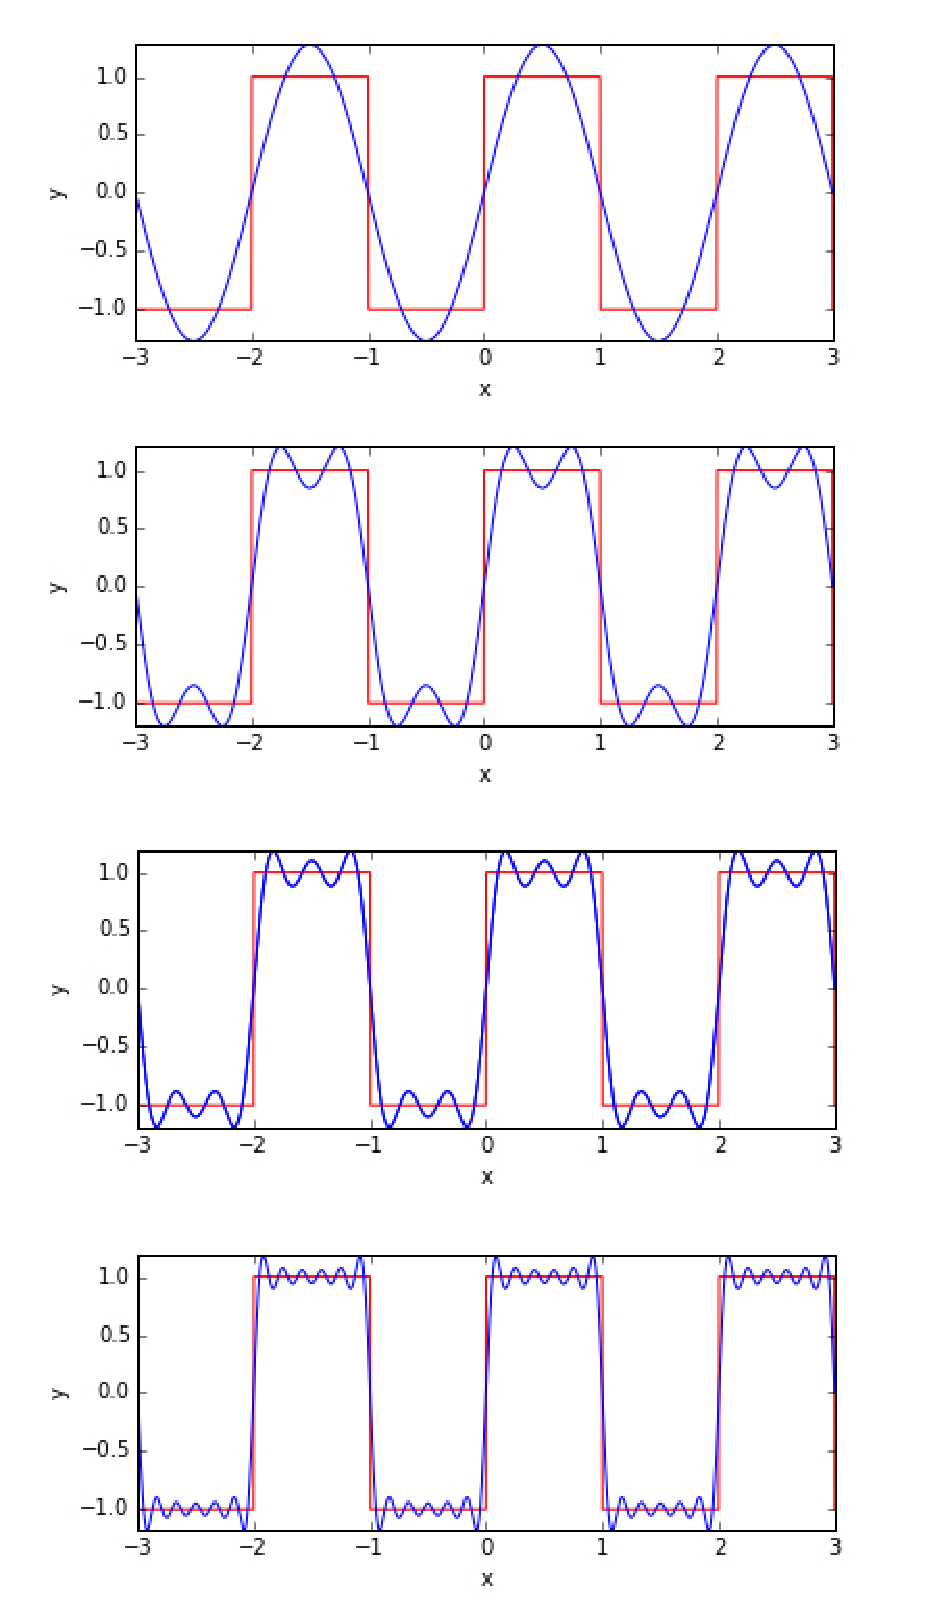
\includegraphics[width=0.40\textwidth]{figs/fsall.pdf}}
\end{center}
\caption{\label{fig:fall} The Fourier Series for a step function including one term, three terms, five terms, and nineteen terms.  The Fourier Theorem states that the series will converge, reproducing the original function, as the number of terms approaches infinity.}
\end{figure}

Just as in the vector analogy, we can determine the Fourier coefficients of a function $f$ by computing the inner products:
\begin{eqnarray*}
A_n = \braket{c_n, f} \\
B_n = \braket{s_n, f}
\end{eqnarray*}
or, in terms of the inner product integrals:
\begin{eqnarray}
A_n &=& \sqrt{\frac{2}{L}} \int_{-\frac{L}{2}}^{\frac{L}{2}} 
f(x) \cos\left(\frac{2\pi n}{L} \, x \right) \, dx \label{eqn:fca} \\
B_n &=& \sqrt{\frac{2}{L}} \int_{-\frac{L}{2}}^{\frac{L}{2}} 
f(x) \sin\left(\frac{2\pi n}{L} \, x \right) \, dx
\end{eqnarray}

Just as in the vector analogy, the inner product determines the correct coefficients only because the basis functions are complete and orthonormal.  We will illustrate this with a function that has all of the $B_n$ equal to zero.  Start with the completeness equation, but change the index from $n$ to $m$ in order to make the next step clearer.  
\begin{displaymath}
f(x) = \sqrt{\frac{2}{L}} \sum_{m=0}^{\infty}  A_m \, \cos\left(\frac{2\pi m}{L} \, x \right)
\end{displaymath}
Now we apply the prescription in Equation~\ref{eqn:fca} to both sides of this equation:
\begin{eqnarray*}
\sqrt{\frac{2}{L}} \int_{-\frac{L}{2}}^{\frac{L}{2}} 
f(x) \cos\left(\frac{2\pi n}{L} \, x \right) \, dx  
&=& \sqrt{\frac{2}{L}} \int_{-\frac{L}{2}}^{\frac{L}{2}} 
\left\{
\sqrt{\frac{2}{L}} \sum_{m=0}^{\infty}  A_m \, \cos\left(\frac{2\pi m}{L} \, x \right) \right\}
\cos\left(\frac{2\pi n}{L} \, x \right) \, dx \\
&=& \sum_{m=0}^{\infty}  A_m \, \left\{ \frac{2}{L} 
\int_{-\frac{L}{2}}^{\frac{L}{2}} 
 \, \cos\left(\frac{2\pi m}{L} \, x \right) \cos\left(\frac{2\pi n}{L} \, x \right) \, dx \right\}\\
&=& \sum_{m=0}^{\infty}  A_m \, \delta_{nm} \\
&=& A_n
\end{eqnarray*}
Note that the last step follows from the fact that, because of the $\delta_{nm}$ in the product, the only non-zero value in the sum across $m$ is the term for $m=n$.

\section{Compact Form of the Fourier Series}

The Fourier Series developed above has the considerable advantage that it makes explicit the role of the sine and cosine functions as an orthonormal basis.  But it is a bit unwieldy as written.  Consider Equation~\ref{eqn:lfs} again:
\begin{eqnarray*}
f(x) = \sqrt{\frac{2}{L}} \sum_{n=0}^{\infty}  A_n \, \cos\left(\frac{2\pi n}{L} \, x \right) + \sqrt{\frac{2}{L}} \sum_{n=1}^{\infty} B_n \, \sin\left(\frac{2\pi n}{L} \, x \right) 
\end{eqnarray*}
Since $\cos(0) = 1$, the first term in the left sum is just a constant $A_0$.  It is also convenient to absorb the normalization factor $\sqrt{2/L}$ into the coefficients.  The series is therefore most often written in the much more compact form:
\begin{eqnarray}
f(x) = a_0 + \sum_{n=1}^{\infty}  \left\{ a_n \, \cos(k_n x ) + b_n \, \sin( k_n x ) \right\}\label{eqn:fs}
\end{eqnarray}
where we have introduced the wave numbers:
\begin{equation}
k_n \equiv \frac{2 \pi n}{L} \label{eqn:kn}
\end{equation}
and the new Fourier Coefficients:
\begin{eqnarray}
a_n &\equiv& \sqrt{\frac{2}{L}}  A_n = \frac{2}{L} \int_{-\frac{L}{2}}^{\frac{L}{2}} 
f(x) \cos( k_n x) \, dx \label{eqn:fca} \\
b_n &\equiv& \sqrt{\frac{2}{L}}  B_n = \frac{2}{L} \int_{-\frac{L}{2}}^{\frac{L}{2}} 
f(x) \sin( k_n x) \, dx \label{eqn:fcb}
\end{eqnarray}


\section{Fourier Series for Complex Functions}

The Fourier Series can be expressed in terms of the complex exponential by noting that:
\begin{eqnarray*}
\cos(k_n x) &=& \frac{\exp(i k_n x) + \exp(-i k_n x)}{2} \\
\sin(k_n x) &=& \frac{\exp.(i k_n x) - \exp(-i k_n x)}{2i}
\end{eqnarray*}
So that Equation~\ref{eqn:fs} can be rewritten as:
\begin{eqnarray}
f(x) &=& a_0 + \sum_{n=1}^{\infty}  \left\{ a_n \, \cos(k_n x ) + b_n \, \sin( k_n x ) \right\} \nonumber \\
&=& a_0 + \sum_{n=1}^{\infty}  \left\{ a_n \,  \frac{\exp(i k_n x) + \exp(-i k_n x)}{2} 
+ b_n \, \frac{\exp(i k_n x) - \exp(-i k_n x)}{2i} \right\} \nonumber \\
&=& a_0 + \sum_{n=1}^{\infty}  \left\{ \frac{a_n - i b_n}{2} \exp(i k_n x) + 
\frac{a_n + i b_n}{2} \exp(-i k_n x) \right\} \nonumber \\
&=& a_0 + \sum_{n=1}^{\infty}  \left\{ c_n \exp(i k_n x) + 
c_n^* \exp(-i k_n x) \right\} \label{eqn:cfsr} \label{eqn:cfsr} 
\end{eqnarray}
Where in the last step we have introduced the complex Fourier coefficient:
\begin{displaymath}
c_n \equiv \frac{a_n - i b_n}{2}.
\end{displaymath}
Note that each term of the sum in Equation~\ref{eqn:cfsr} contains two terms, with the second being the complex conjugate of the first.  Since $z+z^*$ is always a real number, the function $f(x)$ is real valued, as was our initial assumption.

If we replace our initial real function $f(x) $ with a complex valued function $\Psi(x)$ (such as a wave function in Quantum Mechanics!), the constraint that these coefficients are complex conjugates vanishes, and we can replace $c_n^*$ with new independent\footnote{If you prefer, you can construct the complex function from two real functions:  $\Psi(x) = f(x) + i g(x)$.  Either way, you have twice as many independent Fourier coefficients when the function is complex valued.} complex Fourier coefficients $d_n$.   Furthermore, the real constant $a_0$ can be replaced by a complex constant $c_0$.  
\begin{eqnarray*}
\Psi(x)  &=& c_0 + \sum_{n=1}^{\infty}  \left\{ c_n \exp(i k_n x) + 
d_n \exp(-i k_n x) \right\} \label{eqn:cfsr} \label{eqn:cfsr} 
\end{eqnarray*}
And finally, we note that we can simplify this equation even further by being quite clever, noting that 
$k_{(-n)} = -k_n$ and defining $c_{(-n)} \equiv d_n$:
\begin{eqnarray}
\Psi(x)  &=& c_0 + \sum_{n=1}^{\infty}  c_n \exp(i k_n x) + \sum_{n=1}^{\infty}  d_n \exp(-i k_n x) \nonumber \\
 &=& c_0 + \sum_{n=1}^{\infty}  c_n \exp(i k_n x) + \sum_{n=-\infty}^{-1}  c_n \exp(i k_n x) \nonumber \\
\Psi(x) &=& \sum_{n=-\infty}^{\infty} c_n \exp(i k_n x). \label{eqn:cfs}
\end{eqnarray}
Its amusing to compare the size of Equation~\ref{eqn:lfs} with Equation~\ref{eqn:cfs}, and note that the latter form is considerably more powerful.  To determine the complex Fourier coefficients we calculate:
\begin{eqnarray}
c_n &\equiv& \frac{a_n - i b_n}{2}. \nonumber \\
&=& \frac{1}{2} \left\{ 
\frac{2}{L} \int_{-\frac{L}{2}}^{\frac{L}{2}}  \Psi(x) \cos( k_n x) \, dx
-i \frac{2}{L} \int_{-\frac{L}{2}}^{\frac{L}{2}}  \Psi(x) \sin( k_n x) \, dx
\right\} \nonumber \\
&=& \frac{1}{L} \int_{-\frac{L}{2}}^{\frac{L}{2}}  \Psi(x) \left\{\cos( k_n x) - i \sin( k_n x) \right\} \, dx \nonumber \\
c_n &=& \frac{1}{L} \int_{-\frac{L}{2}}^{\frac{L}{2}}  \Psi(x) \exp(-i k_n x) \, dx \label{eqn:cfc}
\end{eqnarray}

Now look closely at Equation~\ref{eqn:cfs} and Equation~\ref{eqn:cfc} and spot the negative sign in the exponential function of the latter.  It seems something strange has happened.  Instead of the sines and cosines, we would like to think of our new orthonormal basis as the complex exponential functions 
\begin{equation}
e_n(x) \equiv \frac{1}{\sqrt{L}}\exp(i k_n x).  
\end{equation}
But to calculate the coefficient of $\exp(i k_n x)$, we integrate with respect to a {\em different} function $\exp(-i k_n x)$.  Can our vector analogy survive this?  It seems as though we are calculating the component along $\hat{x}$ by taking the dot product with $-\hat{x}$.   

It turns out that for complex valued functions, we need to modify our inner product to include complex conjugation of one of the functions:
\begin{equation}
\braket{\Psi, \phi} \equiv \int_{-\frac{L}{2}}^{\frac{L}{2}} \Psi^*(x) \phi(x) \, dx
\end{equation}
With this simple tune up, the vector analogy for complex valued functions is saved!   We still have orthonormal basis functions:
\begin{eqnarray}
\braket{e_n, e_m} &=& \frac{1}{L} \int_{-\frac{L}{2}}^{\frac{L}{2}}  \exp(-i k_n x) \exp(k_m x) \, dx \nonumber \\
&=& \delta_{nm} \label{eqn:eno}
\end{eqnarray}
(you will show this in HW Problem 2) and we still calculate the coefficient of $e_n(x)$ from the inner product:
\begin{equation}
c_n = \frac{1}{L} \braket{e_n, \Psi} = \frac{1}{L} \int_{-\frac{L}{2}}^{\frac{L}{2}}  \Psi(x) \exp(-i k_n x) \, dx
\end{equation}

\section{The Fourier Transform}

The Fourier Series is sufficient for periodic functions.  Unfortunately, this is of rather limited use in physics.  To realize the full potential of the Fourier Theorem, we need to extend the concept to apply to any function, with the only caveat that the function must approach zero as $x$ approaches both negative and positive infinity.

The trick is to consider such a function as periodic with period $L$ in the limit $L \to \infty$.  Recall Equation~\ref{eqn:kn}:
\begin{equation*}
k_n \equiv \frac{2 \pi n}{L}.
\end{equation*}
When $L$ is very large, we will obtain a non-zero value for $k_n$ only for comparably large values of $n$.  But since $n$ is very large, the difference between $k_n$ and $k_{n+1}$ is infinitesimal.  We have moved from the discreet case, where we only have certain wave numbers $k_n$ for each integer $n=0,1,2,...$, to the continuous case, where $k$ can take any real value.  Fortunately, our vector analogy survives intact.

Our inner product now extends between positive and negative infinity:
\begin{equation}
\braket{\Psi, \phi} \equiv \int_{-\infty}^{\infty} \Psi^*(x) \phi(x) \, dx
\end{equation}
Our basis functions, which are now defined for any value of $k$,
\begin{equation}
e_k = \frac{1}{\sqrt{2\pi}} \exp(i k x)
\end{equation}
are still orthonormal, but the condition looks a bit different in the continuum case:
\begin{eqnarray*}
\braket{e_k, e_{k'}} &=& \delta(k-k')
\end{eqnarray*}
See the appendix for more details on the Dirac delta function $\delta(x)$, which is zero everywhere but at $x=0$, where it is infinite.  It is the continuous version of $\delta_{nm}$.

Our basis functions are also still complete.  In the discrete case we have a complex Fourier coefficient for every integer $n$.   Now we have a complex Fourier coefficient for any real value of $k$.  In place of Fourier coefficients, we have instead a function of $k$ which we call the Fourier transform: $\widetilde{\Psi}(k)$.
Instead of a sum over discrete terms, we now have to integrate over all values of $k$:
\begin{equation} \label{eqn:ift}
\Psi(x) = \frac{1}{\sqrt{2\pi}} \int_{-\infty}^{\infty} \widetilde{\Psi}(k) \exp(ikx) \, dk.
\end{equation}
Just as in the discrete case, we determine the Fourier transform from the inner product:
\begin{equation} \label{eqn:ft}
\widetilde{\Psi}(k) = \braket{e_k, \Psi} = \frac{1}{\sqrt{2\pi}} \int_{-\infty}^{\infty} {\Psi}(x) \exp(-ikx) \, dx
\end{equation}
Equation~\ref{eqn:ft} is generally referred to as the {\em Fourier Transform}, while Equation~\ref{eqn:ift} is referred to as the {\em Inverse Fourier Transform}.

\section{The Fourier Transform in Quantum Mechanics}

So far we have been considering the Fourier transform with respect to position $x$ and wave-number $k$.  A much more useful pair of variables for Quantum Mechanics turns out to be momentum $p$ and position $x$.  To relate $p$ to $k$ we need only apply the DeBroglie relation to the wavelength in the definition of the wavenumber:
\begin{displaymath}
k \equiv \frac{2 \pi}{\lambda} = \frac{2 \pi p}{h} = \frac{p}{\hbar}
\end{displaymath}
We could therefore make the substitution $k \to p/\hbar$ (and $dk \to dp / \hbar)$) in Equations~\ref{eqn:ift} and ~\ref{eqn:ft}.  It turns out that a marginally more useful equation results if we make the normalization factors symmetric, by splitting the normalization factor of $1/\hbar$ across both equations with $1/\sqrt{\hbar}$ applied to each:
\begin{eqnarray} 
\Psi(x) &=& \frac{1}{\sqrt{2\pi\hbar}} \int_{-\infty}^{\infty} \widetilde{\Psi}(p) \exp(ipx/\hbar) \, dp \\
\widetilde{\Psi}(p) &=&  \frac{1}{\sqrt{2\pi\hbar}} \int_{-\infty}^{\infty} {\Psi}(x) \exp(-ipx/\hbar) \, dx
\end{eqnarray}
The major benefit of this symmetric form is that the normalization of $\Psi(x)$ and $\widetilde{\Psi}(p)$ in this case turns out to be the same:
\begin{displaymath}
\int_{-\infty}^{\infty} |\Psi(x)|^2 dx = \int_{-\infty}^{\infty} |\widetilde{\Psi}(p)|^2 dp = 1 
\end{displaymath}
Because we can always calculate $\Psi(x)$ from $\widetilde{\Psi}(p)$ either one completely describes the quantum mechanical state.  We call $\widetilde{\Psi}(p)$ the momentum wave function.   Whereas $|\Psi(x)|^2$ gives us the probability density for the quanton to be at position $x$, $|\Psi(p)|^2$ gives us the probability density for the quanton to have momentum $p$.

\section{The Uncertainty Principle}

Imagine that a particle is near $x=0$ with some uncertainty $\sigma_x$.  One way we might describe such a state is that the probability distribution is a Gaussian (bell-curve) distribution:
\begin{displaymath}
|\Psi(x)|^2 = N_x^2 \exp\left(-\frac{x^2}{2\sigma_x^2}\right)
\end{displaymath}
where $N_x$ is a normalization factor chosen such that 
\begin{displaymath}
\int_{-\infty}^{\infty} |\Psi(x)|^2 = 1.
\end{displaymath}
One wave function that would lead to such a probability distribution is 
\begin{displaymath}
\Psi(x) = N_x \exp\left(-\frac{x^2}{4\sigma_x^2}\right).
\end{displaymath}
Let's look at the momentum wave function for this particle:
\begin{eqnarray} 
\widetilde{\Psi}(p) &=&  \frac{1}{\sqrt{2\pi\hbar}} \int_{-\infty}^{\infty} {\Psi}(x) \exp(-ipx/\hbar) \, dx \\
&=&  \frac{N}{\sqrt{2\pi\hbar}} \int_{-\infty}^{\infty}  \exp \left(-\frac{x^2}{4\sigma_x^2} - \frac{ipx}{\hbar}\right) \, dx
\end{eqnarray}
The trick to solving this integral is called {\em completing the square}, we add and subtract the missing term needed to write this as $(x+a)^2 + b$:
\begin{eqnarray*} 
X &=&  -\frac{x^2}{4\sigma_x^2} - \frac{ipx}{\hbar} \\
&=&  -\frac{1}{4\sigma_x^2}(x^2 - 4ipx\sigma_x^2/\hbar) \\
&=&  -\frac{1}{4\sigma_x^2}(x^2 - 4ipx\sigma_x^2/\hbar  + 4i^2p^2\sigma_x^4/\hbar^2 - 4i^2p^2\sigma_x^2/\hbar^2) \\
&=&  -\frac{(x - 2 i p\sigma_x^2/\hbar)^2}{4\sigma_x^2} - p^2\sigma_x^2/\hbar^2
\end{eqnarray*}
The whole point of this is that because $x$ runs from $-\infty$ to $\infty$ we can now make a change of variables $x - 2 i p\sigma_x^2/\hbar \to x$ to clean things up dramatically:
\begin{eqnarray*} 
X &=&  -\frac{x^2}{4\sigma_x^2} - p^2\sigma_x^2/\hbar^2
\end{eqnarray*}
Our integral now becomes:
\begin{eqnarray} 
\widetilde{\Psi}(p) &=&  \frac{N}{\sqrt{2\pi\hbar}} \int_{-\infty}^{\infty}  \exp \left( -\frac{x^2}{4\sigma_x^2} - p^2\sigma_x^2/\hbar^2 \right) \, dx \nonumber \\
&=& \left\{ \frac{N}{\sqrt{2\pi\hbar}} \int_{-\infty}^{\infty}  \exp \left( -\frac{x^2}{4\sigma_x^2} \right) \right\} \exp\left( - p^2\sigma_x^2/\hbar^2 \right) \nonumber \\
&=& N_p \exp(-p^2 \sigma_x^2/\hbar^2) \label{eqn:psip}
\end{eqnarray}
Where in the last step we have noted that the term in brackets is just a constant and set $N_p=\{...\}$.

Fortunately the term in brackets ${}$ does not depend on $p$ at all... there's no need to calculate it, it will just give us a normalized momentum wave function.  We might it as well just set it to $N_p$:
Recall that we started with a wave function which had a Gaussian (bell-shaped) probability distribution with uncertainty $\sigma_x$:
\begin{displaymath}
|\Psi(x)|^2 = N_x^2 \exp\left(-\frac{x^2}{2\sigma_x^2}\right).
\end{displaymath}
We found that the momentum wave function also has a Gaussian probability distribution, if we call the uncertainty on the momentum $\sigma_p$, the probability distribution should have form the same form:
\begin{eqnarray*}
|\widetilde{\Psi}(p) |^2 &=& N_p^2 \exp\left(-\frac{p^2}{2 \sigma_p^2} \right)
\end{eqnarray*}
Comparing this to Equation~\ref{eqn:psip} we conclude:
\begin{displaymath}
\sigma_p = \frac{\hbar}{2 \sigma_x}
\end{displaymath}
or:
\begin{displaymath}
\sigma_x \sigma_p = \frac{\hbar}{2}
\end{displaymath}
Since uncertainties can always be worse than the best case, we have more generally:
\begin{displaymath}
\sigma_x \sigma_p \geq \frac{\hbar}{2}
\end{displaymath}
This is the Heisenberg uncertainty principle of quantum mechanics.  The more precisely the position is determined, the less precisely the momentum is determined, and vice versa.  It is a direct consequence of the wave like nature of matter.

This is optional reading.  A proper mathematical proof of these concepts requires about a one year course.  Fortunately, physicist are generally satisfied with informal proofs of mathematical concepts, because for us the ultimate validation is experiment!



\end{document}




